\documentclass{article}
\usepackage{amsmath, amssymb}
\usepackage{pgfplots}
\usepackage{mathhint}

\begin{document}

% Set the context for this problem - this information appears in the page header
% and helps the hint system understand what material you've covered
\mathhintcontext{
  book=Keith Murray,
  section=Homework 1,
}

\begin{problem}
(10 points) Each of the following differential equations has a single equilibrium point, at $x=0$. For each equation, find the linearization about $x=0$, and explain what you can conclude about the stability of the equilibrium for the nonlinear system. Also determine the stability type for the nonlinear system (e.g., unstable, Lyapunov stable, asymptotically stable).
\begin{itemize}
  \item[(a)] $\dot{x}=-x$
  \item[(b)] $\dot{x}=-x^2$
  \item[(c)] $\dot{x}=-x^3$ 
\end{itemize}

\end{problem}

\begin{solution}
\paragraph{Part (a)}
For the system $\dot{x}=-x$, linearization about $x_0=0$ gives us 
\[ Df(x)=-1 \implies Df(x_0)=-1 \]
resulting in the linearization $\dot{\xi}=-\xi$. Since $Df(x_0)<0$, we can conclude that the system is asymptotically stable.

\paragraph{Part (b)}
For the system $\dot{x}=-x^2$, linearization about $x=0$ gives us 
\[ Df(x)=-2x\implies Df(0)=0 \]
resulting in the linearization $\dot{\xi}=0$. Since $Df(x_0)=0$, we cannot conclude anything about the stability of the equilibrium from linearization.

To determine the stability of the system, note that $f(x)$ is strictly negative. Hence, for negative initial conditions $x(0)<0$, we have
\[ x(t) < x(0) \]
meaning that $x(t)$ is strictly decreasing with no lower bound.

that for any $\epsilon >0$, for all $\delta>0$ such that $|x(0)-0|<\delta$, it is the case that eventually $|x(t^*)|>\epsilon$ for some $t^*$. Hence the system is unstable.

To determine the stability of the system, we can an analytical expression and argue that for at least one initial condition, the system is unstable. Via separation of variables, we can write 
\begin{gather*}
  -\frac{dx}{x^2}=dt \\
  \int -\frac{dx}{x^2}=\int dt\\
  \frac{1}{x}=t+C\\
  x(t) = \frac{1}{t+C}
\end{gather*}
for the initial condition $x(0)=-1$, we have $C=-1$ resulting in the analytic expression 
\[ x(t) = \frac{1}{t-1} \]
where
\[ \lim_{t\to 1}\frac{1}{t-1}=-\infty. \]
Hence, the system is unstable.

\paragraph{Part (c)}
For the system $\dot{x}=-x^3$, linearization about $x=0$ gives us 
\[ Df(x)=-3x^2\implies Df(0)=0 \] 
resulting in the linearization $\dot{\xi}=0$. Since $Df(x_0)=0$, we cannot conclude anything about the stability of the equilibrium from linearization.

To determine the stability of the system, we can use a Lyapunov approach with function $V(x)=x^2$. Clearly, it follows that $V(x_0)=0$ and $V(x)>0$ for $x\neq x_0$. Taking the time derivative of $V(x)$, we have 
\begin{align*}
  \dot{V}(x)&=2x\dot{x}\\
  &=2x(-x^3)\\
  &=-2x^4
\end{align*}
where $-2x^4 <0$ for $x\neq x_0$. Hence, our system is asymptotically stable.

\end{solution}

\clearpage

\begin{problem}
(10 points) Consider the differential equation
\[ \dot{x}=x^{1/3}, \qquad x(0)=0.\]
The origin $x=0$ is an equilibrium point, so one solution is $x(t)=0$.
\begin{enumerate}
  \item[(a)] Find another solution that satisfies $x(0)=0$, but $x(t)\neq 0$ for $t>0$, and therefore conclude that the solution is not unique. (Why does the uniqueness theorem not apply?)
  \item[(b)] Find an infinite family of solutions that satisy the equation with $x(0)=0$.
\end{enumerate}

\end{problem}

\begin{solution}
\paragraph{Part (a)}
Let's separate variables and solve the ODE:
\begin{gather*}
  \int x^{-1/3}dx=\int dt\\ 
  \frac{3}{2}x^{2/3}=t+C\\
  x(t)=\left( \frac{2}{3}\left(t+C\right) \right)^{3/2}
\end{gather*}
For the condition $x(0)=0$, it follows that $C=0$ and we have
\[ x(t)=\left( \frac{2}{3}t \right)^{3/2}.\]
The uniqueness theorem doesn't apply because the derivative of $x^{1/3}$ at $x=0$ is undefined since
\[f'(x)=\frac{1}{3x^{2/3}}. \]
(Local) uniqueness of solutions only apply for (locally) Lipschitz continuous functions, and (locally) continuously differentiable functions imply (local) Lipschitz continuity.

\paragraph{Part (b)}
We can make an infinite family of solutions be defining the following piecewise equation
\[
x(t) = \begin{cases}
    0, & t<t_0 \\
    \left(\frac{2}{3}(t-t_0)\right)^{3/2}, & t \geq t_0
\end{cases}
\]
where we have $x(t_0)=0$ and 
\begin{align*}
  \frac{d}{dt}\left[\left(\frac{2}{3}(t-t_0)\right)^{3/2}\right]&=\frac{3}{2}\left(\frac{2}{3}(t-t_0)\right)^{1/2}\cdot \frac{d}{dt}\left[ \frac{2}{3}(t-t_0) \right]\\
  &=\frac{3}{2}\left(\frac{2}{3}(t-t_0)\right)^{1/2}\cdot \frac{2}{3}\\
  &=\left(\left(\frac{2}{3}(t-t_0)\right)^{3/2}\right)^{1/3}\\
  &=x^{1/3}
\end{align*}
and hence, we still have $\dot{x}=x^{1/3}$.

Given that $t_0$ is arbitrary, our solution 
\[
x(t) = \begin{cases}
    0, & t<t_0 \\
    \left(\frac{2}{3}(t-t_0)\right)^{3/2}, & t \geq t_0
\end{cases}
\]
yields and infinite number of solutions.

\end{solution}

\clearpage

\begin{problem}
(20 points) Consider the system of ODEs given by
\begin{align*}
  \dot{x}&=-y+ax(x^2+y^2)\\
  \dot{y}&=x+ay(x^2+y^2)
\end{align*}
\begin{enumerate}
  \item[(a)] Find all the equilibrium points for this system (for any value of the parameter $a$).
  \item[(b)] Find the equations linearized about $(x,y)=(0,0)$. What does the linearization let you conclude about the stability of the equilibrium point (for the nonlinear system)?
  \item[(c)] Write the system (1) in polar coordinates $(r,\theta)$, with \begin{gather*}
    x=r\cos\theta\\
    y=r\sin\theta
  \end{gather*} and determine the stability type of the equilibrium at the origin. Consider separately the cases $\alpha<0$, $\alpha=0$, and $\alpha>0$.
\end{enumerate}

\end{problem}

\begin{solution}
\paragraph{Part (a)}
Let's start by setting our system equal to zero
\begin{align}
  0&=-y+ax(x^2+y^2)\\
  0&=x+ay(x^2+y^2)
\end{align}
Now multiply equation (1) by $x$ and equation (2) by $y$ to get 
\begin{align*}
  0&=-xy+ax^2(x^2+y^2)\\
  0&=xy+ay^2(x^2+y^2)
\end{align*}
and adding them gives us 
\begin{align*}
  0&=-xy+ax^2(x^2+y^2)+xy+ay^2(x^2+y^2)\\
  &=ax^2(x^2+y^2)+ay^2(x^2+y^2)\\
  &=a(x^2+y^2)(x^2+y^2)\\
  &=a(x^2+y^2)^2
\end{align*}
where if $a\neq 0$, then our only fixed point is the origin $(0,0)$. If $a=0$, then our earlier equations are $\dot{x}=-y$ and $\dot{y}=x$ and the origin is still our only fixed point.


\paragraph{Part (b)}
Our linearization becomes $\dot{\xi}=Df(x_0)\xi$ where $Df(x_0)$ is the jacobian
\[ J_f(x,y) = \begin{bmatrix}
\frac{\partial f_1}{\partial x} & \frac{\partial f_1}{\partial y} \\
\frac{\partial f_2}{\partial x} & \frac{\partial f_2}{\partial y} 
\end{bmatrix} \]
Evaluating each expression, we have 
\begin{gather*}
  \frac{\partial f_1}{\partial x}=a(x^2+y^2)+ax(2x)=ay^2+3ax^3\\
  \frac{\partial f_1}{\partial y}=-1+2axy\\
  \frac{\partial f_2}{\partial x}=1+2axy\\
  \frac{\partial f_2}{\partial y}=a(x^2+y^2)+ay(2y)=ax^2+3ay^3
\end{gather*}
Evaluating each of the expressions at $(0,0)$, we have 
\[Df(x_0)=\begin{bmatrix}
0 & -1 \\
1 & 0
\end{bmatrix} \]
and our linearization is 
\[\dot{\xi}=\begin{bmatrix}
0 & -1 \\
1 & 0
\end{bmatrix}\xi\]
To determine stability, we can compute the eigenvalues via $\det{(A-\lambda I)}=0$.
\[0=\det{(A-\lambda I)}=\lambda^2+1\]
implying that $\lambda=\pm i$ and that we cannot conclude anything about the stability of the equilibrium point.

\paragraph{Part (c)}
Let's start with deriving $\dot{r}$ via the relationship $r^2=x^2+y^2$. We can write 
\begin{gather*}
  \frac{d}{dt}\left[r^2=x^2+y^2\right]\\
  2r\dot{r}=2x\dot{x}+2y\dot{y}
\end{gather*}
and substitute in the values for $\dot{x},\dot{y}$ to get 
\begin{gather*}
  2r\dot{r}=2x\left(-y+ax(x^2+y^2)\right)+2y\left(x+ay(x^2+y^2)\right)\\
  2r\dot{r}=-2xy+2ax^2(x^2+y^2)+2xy+2ay^2(x^2+y^2)\\
  2r\dot{r}=2ax^2(x^2+y^2)+2ay^2(x^2+y^2)\\
  2r\dot{r}=2a(x^2+y^2)(x^2+y^2)\\
\end{gather*}
and substituting in $r^2=x^2+y^2$, we can write 
\begin{gather*}
  2r\dot{r}=2ar^4\\
  \dot{r}=ar^3
\end{gather*}

To derive $\dot{\theta}$, let's differentiate the relationship $\tan\theta=y/x$ to get 
\[ 
  \sec^2\theta \cdot\dot{\theta}=\frac{x\dot{y}-y\dot{x}}{x^2}\\
\]
and plugging in $x^2=r^2\cos^2\theta $, we can write 
\begin{gather*}
  \sec^2\theta \cdot\dot{\theta}=\frac{x\dot{y}-y\dot{x}}{r^2\cos^2\theta}\\
  \sec^2\theta \cdot\dot{\theta}=\frac{x\dot{y}-y\dot{x}}{r^2}\sec^2\theta\\
  \dot{\theta}=\frac{x\dot{y}-y\dot{x}}{r^2}
\end{gather*}
Substituting for $\dot{x},\dot{y}$, we have 
\begin{gather*}
  \dot{\theta}=\frac{x\left(x+ay(x^2+y^2)\right)-y\left(-y+ax(x^2+y^2)\right)}{r^2}\\
  \dot{\theta}=\frac{x^2+axy(x^2+y^2)+y^2-axy(x^2+y^2)}{r^2}\\
  \dot{\theta}=\frac{x^2+y^2}{r^2}\\
  \dot{\theta}=\frac{r^2}{r^2}\\
  \dot{\theta}=1
\end{gather*}

Hence, system (1) in polar coordinates is 
\begin{align*}
  \dot{r}&=ar^3\\
  \dot{\theta}&=1
\end{align*}
To determine the stability type of the equilibrium at the origin, let's consider separately the cases $\alpha<0$, $\alpha=0$, and $\alpha>0$.

For $\alpha<0$, we have $\dot{r}<0$, implying that 
\[||(x(t),y(t))-(0,0)||= \sqrt{x(t)^2+y(t)^2}=r(t)<r(0)= \sqrt{x(0)^2+y(0)^2}=||(x(0),y(0))-(0,0)||\]
Hence, given some $\epsilon>0$, we can set $\delta=\epsilon$ and it follows that for $||(x(0),y(0))-(0,0)||<\delta$ we have 
\[||(x(t),y(t))-(0,0)||< ||(x(0),y(0))-(0,0)||<\delta=\epsilon\]
and 
\[ ||(x(t),y(t))-(0,0)|| < \epsilon.\] 
Furthermore, our reasoning above implies that our trajectories are strictly decreasing and bounded below by the origin. Hence, via the monotone convergence theorem, we can state the as $t\to\infty$ we have $(x(t),y(t))\to (0,0)$ and the origin is asymptotically stable.

For $\alpha=0$, we have $\dot{r}=0$ implying that $r(0)=r(t)$. Hence, we can write 
\[||(x(t),y(t))-(0,0)||= \sqrt{x(t)^2+y(t)^2}=r(t)=r(0)= \sqrt{x(0)^2+y(0)^2}=||(x(0),y(0))-(0,0)||\]
Given some $\epsilon>0$, we can set $\delta=\epsilon$ and it follows that for $||(x(0),y(0))-(0,0)||<\delta$ we have 
\[||(x(t),y(t))-(0,0)||=||(x(0),y(0))-(0,0)||<\delta=\epsilon\]
and
\[ ||(x(t),y(t))-(0,0)|| < \epsilon.\] 
Thus, our system is Lyapunov stable.

For $\alpha>0$, we can solve for $r$ to show that there are initial conditions that result in finite time blow up, showing the origin is unstable. By separating variables, we can write 
\begin{gather*}
  \frac{dr}{ar^3}=dt\\
  \int \frac{dr}{ar^3}=\int dt\\
  -\frac{1}{2ar^2}=t+C\\
  -\frac{1}{2ar^2}=t+C\\
  r(t)=\frac{1}{\sqrt{-2at+D}}
\end{gather*}
For the initial condition $r(0)=1$, we have $D=1$ and the resulting equation 
\[ r(t)=\frac{1}{\sqrt{-2at+1}} \]
experiences finite time blow up as $t\to 1$ given that $a>0$. Hence the origin is unstable.

\end{solution}

\clearpage

\begin{problem}
\noindent
(30 points) The following equations describe the motion of a ball in a spinning circular hoop, where $\alpha$ is the (nondimensional) speed of the spinning hoop, $\beta$ is the (nondimensional) damping, $x$ is the angle of the ball in the hoop, and $y$ is the ball's angular velocity:
\begin{align*}
  \dot{x}&=y\\
  \dot{y}&=(\alpha \cos x-1)\sin x -\beta y,
\end{align*}
\begin{enumerate}
  \item[(a)] Find the equilibrium points, as a function of the parameters $\alpha$, $\beta$ (consider $x\in[-\pi, \pi]$). Make a sketch of these equilibrium points as a function of $\alpha$. (Such a plot is the beginning of a bifurcation diagram).
  \item[(b)] Show that, for $\beta=0$, the system is Hamiltonian: that is, there is a function $H(x,y)$ such that\begin{align*}
    \dot{x}&=\frac{\partial H}{\partial y}\\
    \dot{y}&=-\frac{\partial H}{\partial x}.
  \end{align*}
  \item[(c)] Fix $\alpha=2$, and consider the stability of each of the equilibrium points you found in part (a). Be sure to consider the cases $\beta<0$, $\beta=0$, and $\beta>0$. [\textit{Hint:} How does the Hamiltonian $H$ vary along trajectories $(x(t),y(t))$ that satisfy the dynamics?]
\end{enumerate}

\end{problem}

\begin{solution}
\paragraph{Part (a)}
Let's start by setting everything equal to 0
\begin{align*}
  0&=y\\
  0&=(\alpha \cos x-1)\sin x -\beta y.
\end{align*}
Hence, 
\[0=(\alpha \cos x-1)\sin x\]
We know that $\sin x=0$ when $x=-\pi,0,+\pi$. For the $\alpha \cos x-1$ we can write 
\begin{gather*}
  \alpha \cos x_0-1=0\\
  \cos x_0 = \frac{1}{\alpha}\\
  x_0 =\pm \arccos\frac{1}{\alpha}
\end{gather*}
where $\arccos$ is only defined for inputs in the range of $[-1,1]$. Hence, $x_0$ will only exist when $\alpha\leq -1$ or $\alpha\geq 1$.

Hence, we have at most five equilibrium points at 
\[x_0=-\pi,-\arccos\frac{1}{\alpha},0,+\arccos\frac{1}{\alpha},+\pi\]
with the equilibrium points that depend on $\alpha$ disappearing if $-1<\alpha<1$. Here is a sketch of these equilibrium points as a function of $\alpha$:
\begin{figure}[h]
\centering
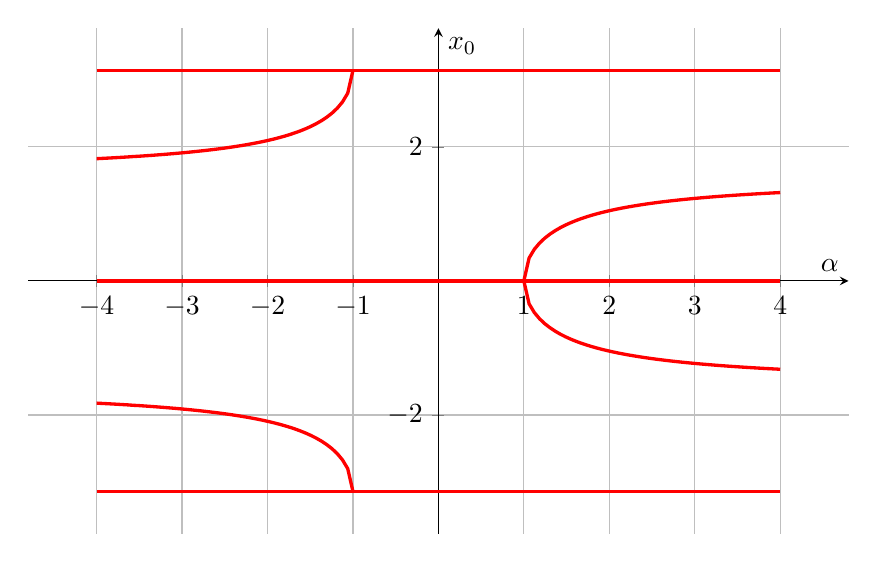
\begin{tikzpicture}
\begin{axis}[
  xlabel={$\alpha$},
  ylabel={$x_0$},
  grid=major,
  width=12cm,
  height=8cm,
  domain=-4:4,
  samples=200,
  axis lines=middle,
  enlargelimits=true,
]
\addplot[red, very thick, domain=1:4, samples=50] {pi*acos(1/x)/180};
\addplot[red, very thick, domain=1:4, samples=50] {-pi*acos(1/x)/180};
\addplot[red, very thick, domain=-4:-1, samples=50] {pi*acos(1/x)/180};
\addplot[red, very thick, domain=-4:-1, samples=50] {-pi*acos(1/x)/180};

\addplot[red, very thick] {0};
\addplot[red, very thick] {-pi};
\addplot[red, very thick] {pi};
\end{axis}
\end{tikzpicture}
\caption{Plot of equilibrium points as a function of $\alpha$}
\end{figure}

\paragraph{Part (b)}
Let's start by writing 
\begin{align*}
  \frac{\partial H}{\partial y} &= y\\
  \int \partial H &= \int y \partial y 
\end{align*}
where integrating both sides with respect to $y$ yields
\[ H(x,y)= \frac{y^2}{2} + f(x). \]
To identify $f(x)$, we can write 
\begin{align*}
  -\frac{\partial H}{\partial x} &= (\alpha \cos x-1)\sin x\\
  \int \partial H &= -\int(\alpha \cos x-1)\sin x \partial x\\
  H(x,y) &= -\int \alpha\cos(x)\sin(x)-\sin x \partial x\\
  H(x,y) &= \int -\alpha\cos(x)\sin(x)\partial x+ \int \sin x \partial x\\
  H(x,y) &=\int-\alpha u\partial u -\cos x + f(y)\\
  H(x,y) &= -\frac{\alpha \sin^2x}{2}-\cos x + f(y)
\end{align*}
and now our Hamiltonian is 
\[ H(x,y)= \frac{y^2}{2}-\frac{\alpha \sin^2x}{2}-\cos x \]

Just as a sanity check, let's compute the partial derivatives to show that this is the correct Hamiltonian. For $\dot{x}$, we can write 
\begin{align*}
  \frac{\partial H}{\partial y}&=y=\dot{x}
\end{align*}
For $\dot{y}$, we can write 
\begin{align*}
  \frac{\partial H}{\partial x}&=-\alpha\sin x \cos x + \sin x\\
  &= -(\alpha\cos x -1)\sin x=-\dot{y}
\end{align*}

\paragraph{Part (c)}
To begin, let's start by performing a linearization. Let's compute $Df(x)$ by writing 
\[ J_f(x,y) = \begin{bmatrix}
\frac{\partial f_1}{\partial x} & \frac{\partial f_1}{\partial y} \\
\frac{\partial f_2}{\partial x} & \frac{\partial f_2}{\partial y} 
\end{bmatrix} \]
Evaluating each expression, we have 
\begin{gather*}
  \frac{\partial f_1}{\partial x}=0\\
  \frac{\partial f_1}{\partial y}=1\\
  \frac{\partial f_2}{\partial x}=(-2\sin x)\sin x + (2\cos x -1)\cos x=-2\sin^2x+2\cos^2x-\cos x\\
  \frac{\partial f_2}{\partial y}=-\beta
\end{gather*}
where we will say $g(x)=-2\sin^2x+2\cos^2x-\cos x$. Hence we have 
\[ A = \begin{bmatrix}
0 & 1 \\
g(x) &  -\beta
\end{bmatrix} \]
and computing 
\[ \det\left(A-\lambda I\right)=0\] 
we have
\[ -\lambda(-\beta-\lambda)-g(x)=0 \]
and can write 
\[ \lambda = \frac{-\beta\pm\sqrt{\beta^2+4g(x)}}{2}. \]
Let's now compute $\lambda$ for each of our equilibria as a function of $\beta$. For $a=2$, we have $\arccos(1/2)=\pi/3$ and we can write 
\begin{center}
\begin{tabular}{c c c c c} 
 $(-\pi,0)$ & $(-\pi/3,0)$ & $(0,0)$ & $(\pi/3,0)$ & $(\pi,0)$ \\[0.5ex] 
 \hline\hline
 $\frac{-\beta\pm\sqrt{\beta^2+4\cdot 3}}{2}$ & $\frac{-\beta\pm\sqrt{\beta^2+4\cdot (-1.5)}}{2}$ & $\frac{-\beta\pm\sqrt{\beta^2+4\cdot 1}}{2}$ & $\frac{-\beta\pm\sqrt{\beta^2+4\cdot (-1.5)}}{2}$ & $\frac{-\beta\pm\sqrt{\beta^2+4\cdot 3}}{2}$ \\ 
\end{tabular}
\end{center}

Now for our equilibria $(-\pi,0),(0,0),(\pi,0)$, we have that our square root quantities ($\sqrt{\beta^2+4\cdot 3}$ and $\sqrt{\beta^2+4\cdot 1}$) are always real and are greater than $|\beta|$. This implies that these equilibria will have at least one positive eigenvalue for all values of $\beta$; hence, $(-\pi,0),(0,0),(\pi,0)$ are unstable for all values of $\beta$.

For our equilibria $(-\pi/3,0),(\pi/3,0)$, the reasoning is more delicate. Let's handle it piecewise.

Let's assume that $\beta>0$. Then we have three cases: $|-6|>\beta^2,|-6|<\beta^2,|-6|=\beta^2$. For the $|-6|=\beta^2$ case, we have $\sqrt{\beta^2-6}=0$ and the equilibria have strictly negative eigenvalues, implying they are asymptotically stable. For the $|-6|>\beta^2$ case, we have $\sqrt{\beta^2-6}$ is an imaginary number and the equilibria have eigenvalues with a strictly negative real part, impying they are asymptotically stable. For the $|-6|<\beta^2$ case, it follows that $|\beta|>\sqrt{\beta^2-6}$, which allows us to write 
\[ -\beta+\sqrt{\beta^2-6}<0 \qquad\text{and}\qquad -\beta-\sqrt{\beta^2-6}<0 \]
Thus the equilibria have eigenvalues with a strictly negative real part, impying they are asymptotically stable. Therefore, in three cases for $\beta>0$, it follows that $(-\pi/3,0),(\pi/3,0)$ are asymptotically stable equilibria.

Let's now assume that $\beta<0$. Then we (again) have three cases: $|-6|>\beta^2,|-6|<\beta^2,|-6|=\beta^2$. For the $|-6|=\beta^2$ case, we have $\sqrt{\beta^2-6}=0$ and the equilibria have strictly positive eigenvalues, implying they are unstable. For the $|-6|>\beta^2$ case, we have $\sqrt{\beta^2-6}$ is an imaginary number and the equilibria have eigenvalues with a strictly positive real part, impying they are unstable. For the $|-6|<\beta^2$ case, it follows that $|\beta|>\sqrt{\beta^2-6}$, which allows us to write 
\[ -\beta+\sqrt{\beta^2-6}>0 \qquad\text{and}\qquad -\beta-\sqrt{\beta^2-6}>0 \]
Thus the equilibria have eigenvalues with a strictly positive real part, impying they are unstable. Therefore, in three cases for $\beta<0$, it follows that $(-\pi/3,0),(\pi/3,0)$ are unstable equilibria.

Let's now assume that $\beta=0$. This is the tricky part, because we get the following expression:
\[ \lambda = \frac{\pm\sqrt{-6}}{2} \]
and we can't conclude anything from the linearization because the real part of our eigenvalues are zero. To make conclusions about the stability, we can turn to the Hamiltonian. As a reminder, with $\alpha=2$, the Hamiltonian is 
\[ H(x,y)= \frac{y^2}{2}- \sin^2x-\cos x \]

First let's evaluate the Hamiltonian at our equilibria to get
\begin{align*}
  H\left(-\pi,0\right)&=\frac{0^2}{2}-\sin^2(-\pi)-\cos(-\pi)=1\\
  H\left(-\frac{\pi}{3},0\right)&=\frac{0^2}{2}-\sin^2(-\pi/3)-\cos(-\pi/3)=-\left(-\frac{\sqrt{3}}{2}\right)^2-\frac{1}{2}=-\frac{5}{4}\\
  H\left(0,0\right)&=\frac{0^2}{2}-\sin^20-\cos0=-1\\
  H\left(\frac{\pi}{3},0\right)&=\frac{0^2}{2}-\sin^2(\pi/3)-\cos(\pi/3)=-\left(\frac{\sqrt{3}}{2}\right)^2-\frac{1}{2}=-\frac{5}{4}\\
  H\left(\pi,0\right)&=\frac{0^2}{2}-\sin^2(\pi)-\cos(\pi)=1
\end{align*}
These values imply that the Hamiltonian has a global minimum of $-\frac{5}{4}$, so in order to make a Lyapunov, we can write 
\[ V(x,y)=\frac{y^2}{2}-\sin^2x-\cos x+\frac{5}{4} \]
Here, it is obvious that $V\left(-\frac{\pi}{3},0\right)=0$ and $V\left(\frac{\pi}{3},0\right)=0$, and that $V>0$ elsewhere. Differentiating our function with respect to time (with $\alpha=2$), we have
\begin{align*}
  \frac{d}{dt}V(x,y)&=y\dot{y}+\left( -2\sin x\cos x +\sin x \right)\dot{x}\\
  &=\left((2 \cos x-1)\sin x -\beta y\right)y - \left(2 \cos x-1\right)\sin x \cdot y\\
  &=(2 \cos x-1)\sin x\cdot y -\beta y^2 - \left(2 \cos x-1\right)\sin x \cdot y\\
  &=-\beta y^2
\end{align*}
and since we have $\beta=0$, it follows that $\dot{V}=0$ everywhere.

From this, we can conclude that for $\beta=0$, the equilibria $(-\pi/3,0),(\pi/3,0)$ are Lyapunov stable. In fact, this makes sense because the derivative of the Hamiltonian being equal to zero implies that orbits travel on level sets. Hence, the equilibria $(-\pi/3,0),(\pi/3,0)$ are centers with trajecories starting sufficiently close to them oscillating around them.

To recap, for all values of $\beta$, we have the following stabilities 
\begin{center}
\begin{tabular}{ |c|c|c|c|c|c| } 
 \hline
  & $(-\pi,0)$ & $(-\pi/3,0)$ & $(0,0)$ & $(\pi/3,0)$ & $(\pi,0)$\\
 \hline
 $\beta >0$ & unstable & asymptotically stable & unstable & asymptotically stable & unstable \\ 
 $\beta =0$ & unstable & Lyapunov stable & unstable & Lyapunov stable & unstable \\ 
 $\beta <0$ & unstable & unstable & unstable & unstable & unstable \\ 
 \hline
\end{tabular}
\end{center}

\end{solution}

\clearpage

\begin{problem}
\noindent
(30 points) Use the candidate Liapunov function
\[ V(x,y)=\frac{1}{2}y^2+(1-\cos x) \]
to show that the origin $(x,y)=(0,0)$ is a locally asymptotically stable fixed point for the system
\begin{align*}
  \dot{x}&=y\\
  \dot{y}&=-\epsilon y^3-\sin x
\end{align*}
whenever $\epsilon>0$.

\end{problem}

\begin{solution}

Let's start by showing that our candidate Liapunov function has the desired properties. To show that $V(0,0)=0$, we write 
\[ V(0,0)=\frac{1}{2}(0)^2+(1-\cos 0)=0+(1-1)=0. \] 

To show that $V(x)>0$ for all $x\neq x_0$, let's consider a region
\[ U=\left\{ (x,y)\in\mathbb{R}^2 : x\in[-\frac{\pi}{2},\frac{\pi}{2}] \text{ and } y\in[-1,1] \right\} \]
in order to exclude points like $(2\pi,0)$ where $V(2\pi,0)=0$. Our $y$ portion of $V$ will remain strictly positive when $y\neq 0$, and our $x$ portion ($1-\cos x$) will remain strictly positive when $x\in[-\frac{\pi}{2},\frac{\pi}{2}]$. Hence, $V(x,y)>0$ for all $(x,y)\neq (0,0)$.

To show that $\dot{V}(x,y)\leq 0$ for $(x,y)\neq (0,0)$, let's take the derivative. We write 
\begin{align*}
  \frac{d}{dt}V(x(t), y(t))&=\sum_{i=1}^{n}\frac{\partial V}{\partial x_i}\dot{x}_i\\
  &=(\sin x)\dot{x}+y\dot{y}\\
  &=(\sin x)y+y(-\epsilon y^3-\sin x)\\
  &=(\sin x)y -\epsilon y^4 - (\sin x)y\\
  &=-\epsilon y^4 
\end{align*}
and given that $\epsilon>0$, we can conclude that $\dot{V}=-\epsilon y^4\leq 0$. However, this only proves that our system is Lyapunov stable and not asymptotically stable. To show asymptotic stability, we can invoke La Salle's invariance principle, as we did in lecture 2.

Consider the set 
\[ S=\left\{(x,0): x\in\left[-\frac{\pi}{2},\frac{\pi}{2}\right]\right\} \]
where it follows that $\dot{V}(x,y)=0$ for every $(x,y)\in S$. Yet, for trajectories that either start in or intersect the set at a point where $x\neq 0$, we have $\dot{y}=-\sin x\neq 0$, implying that part of the future trajector will leave the set. Hence, the only trajectory in $S$ that is invariant under our system is the trivial trajectory of $(x(0),y(0))=(0,0)$, and we can invoke LaSalle's invariance principle to argue that the origin is a locally asymptotically stable fixed point.

\end{solution}

\end{document}